To the best of our knowledge, Golden Gate~(originally MIDAS II) is the first
open-source, optimizing FAME compiler. The content in this chapter loosely
mirrors that of our 2019 ICCAD publication~\cite{GoldenGate}, but better
contextualizes the design of the compiler against MIDAS; describes features,
like target-to-host bridges, not discussed in the ICCAD publication; and
elaborates on implementation details pertinent to the later chapters of this
dissertation.  For a second perspective, with expanded discussion on the
optimizations themselves and how they were verified, we direct the interested
reader to Albert Magyar's dissertation. Code references in this chapter will
refer to sources in FireSim version
1.8.0\footnote{https://github.com/firesim/firesim/tree/1.8.0}.

\section{Design Objectives}

We had the following objectives in mind when we set to redesign MIDAS:

\begin{enumerate}
\item \textbf{Maintain FireSim feature completeness.} We wanted the ability to
drop in Golden Gate as a replacement for MIDAS in a future FireSim release, with the
only user-facing difference being the availability of new
optimizations. As a side effect of a more sophisticated compiler we expected
compile times would increase, however, we wanted unoptimized simulators to have
approximately the same perfomance and resource utilization as those generated by MIDAS.

\item \textbf{Minimize user modification of ASIC RTL.} It is all too easy to
provide a crutch the compiler by requiring the user make RTL changes to expose
optimization opportunities. The difficulty is these changes can be
invasive: they may introduce new bugs, adversly affect ASIC QoR, or worsen source maintainability. While we expect there
may be times where these sorts changes are desired, we made no such
changes in the Rocket Chip or BOOM codebases to implement the optimizations
described in our ICCAD paper.

\item \textbf{Provide a mechanism to rigorously verify the optimizations.} RAMP-style, multi-cycle resource optimizations introduce considerable complexity into the
simulator, making the resulting system harder to debug
effectively. A buggy optimization can introduce simulation deadlock or false
bugs in the target design.
More insidiously, an optimization may produce a functionally correct simulator with slightly
different target-timing behavior~(e.g., a latency insenstive transaction may be delayed an extra cycle), introducing difficult-to-detect performance
descrepancies. We wanted users to trust the compiler wasn't changing their
design beneath their feet.

\item \textbf{Enable the use of FireSim as a library for hardware emulation.}
MIDAS and FireSim had developed in isolation of the chip-design projects
ongoing at UCB-BAR, and used custom forks of many of the same hardware and
target-software libraries. This made it challenging for chip designers to run
their designs in FireSim without help from a FireSim developer to make their design ``FireSim-compatible". We
wanted to make it possible to include FireSim in a chip-like project---specifically, in what would
would become Chipyard~\cite{Chipyard}---to support seemlessly pushing real
designs through an emulation flow.
\end{enumerate}

Our desire to maintain FireSim feature completeness made it clear from the
outset that a complete redesign of the compiler was untenable in a reasonable timeframe. Instead, Golden
Gate was developed as a series of reimplementations of key phases of
MIDAS. This let us continually build functional emulators of the same designs
supported in mainline FireSim. We started with introducing support for
optimizations, while maintaining the existing endpoint support and compiler
interface~(described in Sections~\ref{sec:midas-endpoints} and \ref{sec:midas-chisel-api}
respectively).

To enable optimizations, we considered a few possibilities such as: leaning on
the endpoint system and user modifications to the target RTL (this violates
objective two); or using specialized transformations to implement optimizations
directly as modifications to the hub model~(this made it more difficult to
achieve objective three).  Ultimately, what we settled on was a LI-BDN-based compiler organization that leverages extensive target module-hierarchy modifications to
wrap and isolate optimization candidates in their own modules. These modules become the reference SSMs for each unit. They can be FAME
transformed into a primitive LI-BDN and successively reimplemented without consideration with how they are connected
to the rest of the simulator. Then, the unit and its corresponding reference module can be fed into a
verification flow to show the resulting unit satisfies PI. In principle, this could be applied to every unit-SSM pair in the network to
show the simulator is a valid LI-BDN implementation of the complete source design.

LI-BDN removes the explicit need for channels and permits modules (and thus resulting units) to be
combinationally coupled, widening the scope of potential optimizations. While we
acknowledge that forcing optimizations to apply only at registered boundaries
between units~(a requirement of a channel-bootstrapped formalism) would
produce simulators that sustain greater FMRs, this would add complexity to the
compiler and could make many optimizations infeasible. We also note that these
sorts ``channel-like`` of optimizations are not fundamentally precluded by the LI-BDN formalism. For example, when an edge
between two units is driven by an output port with no combinational dependency on
an input, it may be possible to implement that edge using a flow-through queue to save a
cycle of transmission latency.

Moving to an LI-BDN formalism resolves a number of other modeling
challenges MIDAS users face.  Requiring that non-wire-channels be injected
between endpoints and the hub unit is too restrictive in some cases where
the user wishes to model a combinational path that propagates through an
endpoint. Another challenge was defining the reset semantics of these
stateful channels.  MIDAS relies on FPGA programming to properly initialize
these channels, however they are not held in target reset during
simulation: it is purely coincidental that the hub unit does not
spuriously enqueue target data into queue-type channels while parts of the
hub are under target reset. For a time, MIDAS would broadcast target reset
tokens to channels and endpoints, but this too is fraught, as resets driving
registers in the hub maybe different from this special-cased global reset.
Instead of requiring that user specify this reset for each channel, LI-BDN
can sidestep these issues entirely by removing the need for stateful
channels and allowing the compiler to assume fewer things about target.

The second phase of Golden Gate's development addressed the fourth objective,
and required a redesign of the compiler interface and endpoint system. Here, we
decoupled Golden Gate from target elaboration: Golden Gate accepts a FIRRTL
file and annotations. \emph{Target-to-Host Bridges}, or bridges for
short, replace endpoints and are instantiated throughout the target module
hierarchy during target elaboration. Unlike MIDAS, Golden Gate does not match
on the Chisel I/O of the top-level module. Instead, it finds annotations~(\texttt{BridgeAnnotations}) bound to the aforementioned modules that provide the
class name of a Chisel generator Golden Gate should invoke to replace the black
box.

\section{Compiler Input \& Target Specification}

Golden Gate accepts a ``closed" description of the target
consisting of FIRRTL and annotations. We show a pictoral example of this using
typical Chipyard-generated SoC in Figure~\ref{fig:gg-target}. By closed, in
this case we mean that the top-level module has no I/O: the user instantiates their chip in a top-level
environment or harness module and drives the chip-interfaces using target-RTL
or, if that is insufficient, bridges. Bridges are so named because they span
the host and target domains. The \emph{target side} of a bridge consists of a
Chisel module, generally a black box, whose instance is annotated with a bridge annotation,
and whose ports are annotated to specify how the
interface should divided into token streams. The \emph{host side} of a bridge is a unit (a
primitive LI-BDN) that implements that blackbox module. Just like an endpoint,
the host-side unit consists of a module (\emph{BridgeModule}) and a driver
(\emph{BridgeDriver}). Finally, to enable optimizations, users
identify specific structures in the target by annotating them. As in MIDAS, additional compiler-side features are controlled using a
parameters instance which enables instrumentation passes and configures host-platform support.
Additional user-supplied host and target FIRRTL transforms are provided in this parameters instance.

\begin{figure}
    \centering
    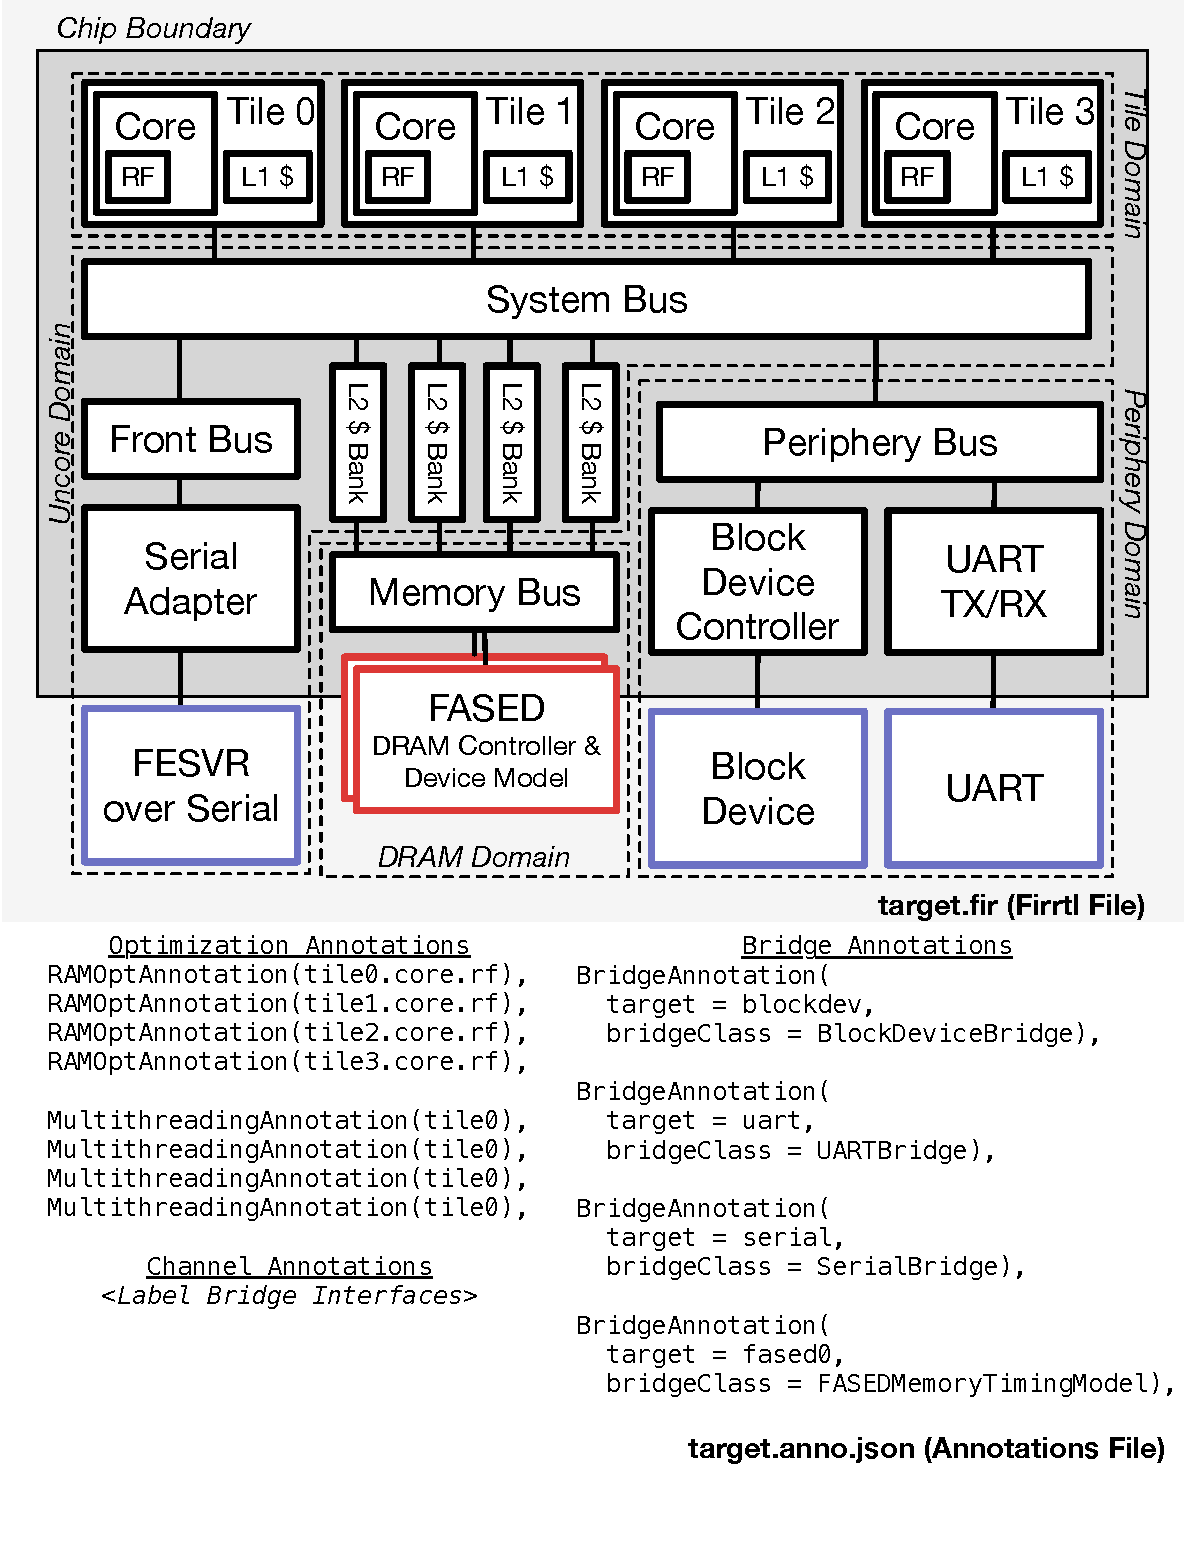
\includegraphics[width=0.99\textwidth]{figures/gg-target.pdf}
    % graffle2pdf -c gg-target midas-graphics/graffle/midas2-target.graffle figures/gg-target.pdf
    \caption{A typical Chipyard SoC passed to Golden Gate (top), and its associated Golden Gate specific
    annotations (bottom). Clock domains are shown for reference in later chapters.}
    \label{fig:gg-target}
\end{figure}

Since it does not require access to unserializable Scala
types like MIDAS, Golden Gate can be invoked as standalone application on an
elaborated target. This permits running the
compiler on a target elaborated in a different environment that may include a
different version of Chisel, FIRRTL, and Rocket Chip than those the compiler
itself depends on. We give an example invocation of Golden Gate in Listing~\ref{lst:gg-invocation}.

\begin{lstlisting}[style=shell, language=bash, label={lst:gg-invocation}, caption=An example command-line invocation of Golden Gate.]
  sbt runMain midas.stage.GoldenGateMain \
      -o <output filename> \
      -td <output directory> \
      -i  <input FIRRTL filename> \
      -faf <input FIRRTL annotations file> \
      -ggcp <Golden Gate parameters scala package> \
      -ggcs <Golden Gate parameters scala class string> \
      -E verilog
\end{lstlisting}

\section{Updated Compiler Flow}

We show a depiction of Golden Gate's compilation flow and how modifies an
illustrative toy-design in figure~\ref{fig:gg-toolchain}.  We omitt
debug-synthesis transforms, and user-provided transformations for brevity.
Golden Gate tranformations, which are statically ordered in
\texttt{MidasTransforms}\footnote{See sim/midas/src/main/scala/midas/passes/MidasTransforms.scala}, can be
roughly\footnote{Note, these terms are not currently enshrined in the
codebase.} divided into three phases:

\begin{figure}
    \centering
    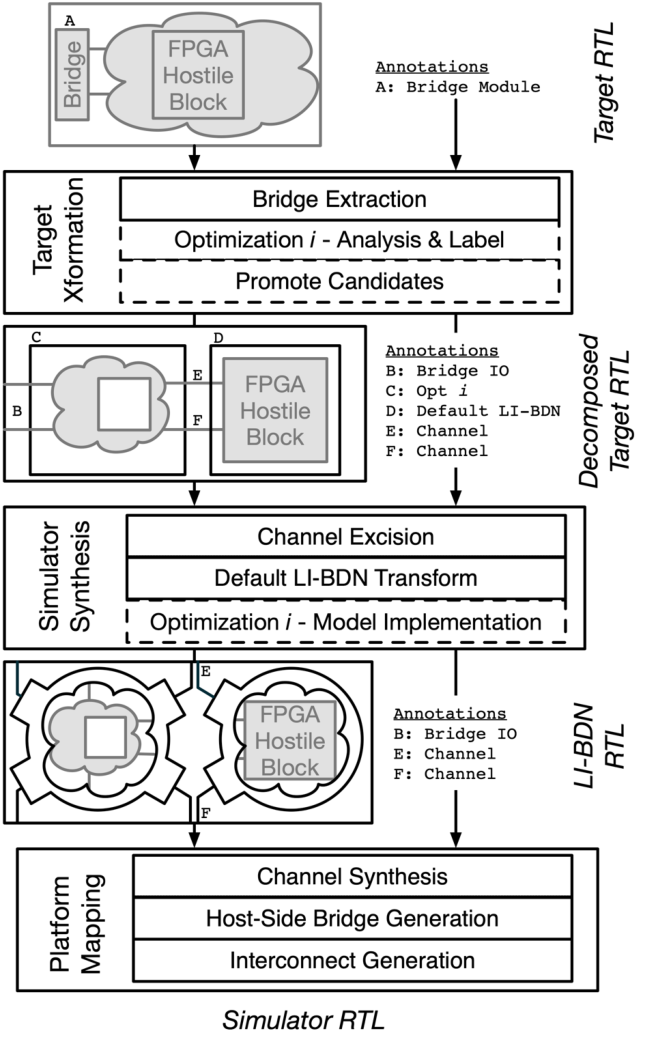
\includegraphics[width=0.8\textwidth]{figures/gg-toolchain.pdf}
    \caption{Core phases of the Golden Gate compiler and a high-level depiction
    of the transformations made to the underlying target and its annotations. The default LI-BDN transform
    is the FAME1 transform.}
    \label{fig:gg-toolchain}
\end{figure}

\begin{enumerate}

\item \textbf{Target Transformation.} Here the
module hierachy is mutated in preperation for host decoupling. Bridges are
extracted and unsynthesizable debugging constructs are replaced and
bound to a bridge interface. Primitives identified for optimization are
wrapped in modules and labelled with additional optimization annotations. These are then promoted to the top of the design hierarchy. 
All top-level modules instances correspond to units in the eventual
simulator and top-level connectivity define edges in the graph.

\item \textbf{Simulator Synthesis.} Here top-level modules are transformed
into, or replaced with, primitive LI-BDN units. On completion, the output circuit consists of a
series of unconnected unit instances. Connectivity between units is captured in
channel annotations between top-level I/O.

\item \textbf{Platform Mapping.} This consists of the Simulation Mapping and
Platform Mapping passes of MIDAS. A chisel-generated wrapper includes all
channel implementations and elaborated host-side bridge modules. The resulting output
circuit is compatible with the same FPGA projects as MIDAS-generated
simulators and plugs directly into FireSim's existing build flow.
\end{enumerate}

\subsection{Annotations}
Golden Gate relies on FIRRTL's annotation system to communicate information about the
circuit from transform-to-transform instead of an auxiliary
datastruture that persists across transformations. The main motivation for doing so was to make transforms in the
compiler robust against running lowering or optimization transformations
between them. The FIRRTL compiler framework provides callbacks for defining
how annotations should be modified when the circuit structures an annotation targets are
changed (a process known as \emph{renaming}). We describe the key annotations here:

\begin{itemize}
    \item \textbf{Bridge Annotations}~(\texttt{BridgeAnnotation}) label module
        instances in the target for which a custom unit will be generated.  In
        addition to labelling a target module instance, they carry a fully qualified
        class name of the Bridge Module to be generated and its optional
        constructor parameter. Finally, the annotation enumerates the names of all
        of its channel annotations.

\item \textbf{Connection Annotations}~(\texttt{FAMEChannelConnectionAnnotation}), or \emph{channel} annotations, label connections between modules that correspond to units and bridges of the simulator, and
    carry the information required to generate a channel them. This consists of
    a list of sources~(\texttt{sources}), I/O fields on the instance that drives the connection
    (i.e., they source the tokens), and sinks~(\texttt{sinks}), I/O fields on an instance
    receiving those connections. Channels carry additional metadata,
    including a globally unique string identifier~(\texttt{globalName}), as well as a case class~(\texttt{chInfo}) that
    captures target properties of connection and channel-implementation hints.
    The \texttt{chInfo} has subtypes to indicate whether the channel is latency
    insensitive and should be implemented with a queue-type channel, or is a pipe-type channel.

\item \textbf{Port Annotations}~(\texttt{FAMEChannelPortAnnotation}) label groups of I/Os in a module as corresponding to a channel source or sink.
    The list of sources or sinks in connection annotations (which point
    at instances of the module) must agree with the port annotation on the
    module itself. Port annotations are primarly consumed by transformation passes and provide the simplest means
    to look up how the I/Os of the module should be divided into channels.

\item \textbf{Model Annotations}~(\texttt{FAMEModelAnnotation}) serve a similar function to BridgeAnnotations, in that they label a
    module as being a unit. Unlike bridges, instances of the target module
    are not extracted from the design hierarchy but instead are promoted to
    the top-most level of the design hierarchy, so that they can later be
    transformed by the compiler in Simulator Synthesis.
\end{itemize}

At the start of compilation, bridge annotations are present, with connection
annotations labelling each bridge's interfaces\footnote{We note this is an abuse of the
abstraction presented by the annotation~(described above), which is fully realized only once bridges are extracted.}
Model annotations may also present alongside specific optimization annotations.

\section{Target Transformation}

The primary function of Target Transformation is to coerce the design's module
hierarchy into a form that matches the eventual simulator topology: top-level
instances, which wrap optimization candidates, map to unit instances~(nodes) and top-level connections map to
channels~(edges). Throughout this process, no host-time simulator constructs
are introduced: the RTL still directly represents the chip, albeit with a different module hierarchy.  Target Transformation
consists of all transformations before top-level connectivity is removed
(\texttt{ChannelExcision}).

Target Transformation commences with an initial lowering and optimization of the input FIRRTL, after which
the input circuit is checked for Golden Gate compatibility (namely, the circuit
presents no top-level I/O; see \texttt{EnsureNoTargetIO}). Next, Golden Gate
runs assertion and printf synthesis. Under-the-hood these do not fundamentally differ
from what was described in our DESSERT publication~\cite{DESSERT}, however
synthesized debug primitives are now bound to bridges~(more on this later).

Now Golden Gate finds all modules annotated with a bridge annotation and extracts
them~(\texttt{BridgeExtraction}). Connections to instances of
a bridge are replaced with connections to newly added
top-level I/O. Note that a single bridge module with $N$ instances will produce $N$
sets of ports at the top-level. The bridge and connection annotations are
"promoted" to point at these new top-level interfaces. Bridge annotations are then
replaced with a form of annotation that targets top-level I/O
(\texttt{BridgeIOAnnotation} instead of a module but are otherwise indentical.
Finally, connection annotations are assigned new \texttt{globalNames} to ensure they
are unique and their corresponding bridge annotations are updated to reflect
that.

Next, Golden Gate prepares for its optimization-focused hierarchy manipulations
by adding a wrapper module, the \emph{FAME wrapper}, around the existing
design~(\texttt{WrapTop}). Once optimization candidates have been removed, the
previous top-level module will become the central "hub" unit in the simulator.

It is at this point we envisioned custom optimization analyses would be run
find and label optimization opportunities. Currently, the multi-ported RAM
analysis is only example of this in the code base~(see
\texttt{LabelSRAMModels}).  This pass finds FIRRTL memories that have been
annotated as safe to optimize, wraps them in a module, and labels them with a
model annotation.

Then Golden Gate finds all module instances labeled with a model annotation, and
promotes them to the FAME wrapper. This process is nearly identical
to bridge extraction, but the module is not completely removed. Just as in
bridge extraction, one annotated model will produce as many top-level instances
as there were instances of the module in the design hierarchy.  At this point
the connectivity within the wrapper reflects the star-topology of the eventual
simulator: the original source module is the hub and all promoted modules and
bridge interfaces connect directly to it.

With the module hierarchy manipulations finished, Golden Gate completes Target
Transformation by fleshing out missing annotations~(\texttt{FAMEDefaults}). This primarily consists of labelling
all inter-model connectivity with connection annotations. This pass makes no
attempt to group connections into a single channel: each ground-type
connection between the hub and a spoke gets its own annotation and thus will receive an independent channel implementation.

\section{Simulator Synthesis}

Simulator Synthesis is so named because it begins introducing host-time constructs into the circuit,
most notably with the execution of the default FAME1 transformation. Simulator
Synthesis begins by removing all inter-model connectivity and replacing it
with top-level I/O~(\texttt{ChannelExcision}). Connection annotations are
promoted to point at these new interfaces. Only now are port annotations
added~(\texttt{InferModelPorts}), since connections between nodes (both bridges and models)
now uniformly target top-level I/O.  This transformation
ensures that connection annotations on instances of the same module agree as to how
ports correspond to channels. Since \texttt{FAMEDefaults} makes no attempt to
group channels currently, this mainly serves as a consistency check on
bridge-bound channels and ensures no connection annotations have been lost.

The bulk of the complexity in Simulator Synthesis is contained in its default
FAME1 transform (\texttt{FAMETransform}). It has two fundamental tasks: first, it
transforms all top-level modules, including those that will be optimized later,
into units using a default, wrapper-based LI-BDN transform~(described
previously and shown in Figure~\ref{fig:libdn-wrapper}). The transform groups
ports into new decoupled interfaces by consuming the port annotations for the module under transformation.
References to target ports are replaced with references to the payloads
of these decoupled channel ports. Valid and ready signals are used to build out the
control circuitry shown in Figure~\ref{fig:libdn-wrapper}, however,
this logic is appended to the existing module (to avoid introducing another
level into the module hierarchy). Finally, all references to the target clock
are replaced with references to the output of a clock buffer which is responsible for driving a selectively
gated target clock.  The clock
buffer itself is left as a black box that will be implemented later for the
desired host FPGA.  The second major function of the FAME transform is to
rewire the FAME wrapper by replacing existing I/O and connectivity with decoupled
equivalents. For example, a boolean driven by a model is replaced with a three
bit interface: valid and the boolean payload is driven by the model, and ready
is driven by the I/O interface in the FAME wrapper. Connection annotations are
updated to point at the payloads of these channels.

At this point, Golden gate runs optimization transformations to replace the
default unit implementations. Since the default FAME
transformation has already decoupled the interfaces of the reference SSM, these
transformations simply replace the module body of the existing primitive LI-BDN.
Connectivity in the FAME wrapper remains unchanged.  Simulator Synthesis
concludes with some fix-up transformations which provide a default clock buffer
implementation (\texttt{DefineAbstractClockGate}) compatible with RTL
simulators, and wire up the host-clock and reset to all units in the FAME
wrapper(\texttt{ConnectHostClock}).

\section{Platform Mapping}\label{sec:gg-platform-mapping}

In Golden Gate, platform mapping is responsible for implementing all
channels (previously, known as simulation mapping in MIDAS) and elaborating
all remaining simulation collateral, such as bridges and resource interconnect
(previously, platform mapping in MIDAS). This happens in single Chisel
invocation, and produces three layers of wrapper modules, shown in Figure~\ref{fig:sim-wrapper-layers}.

\begin{figure}
  \centering
    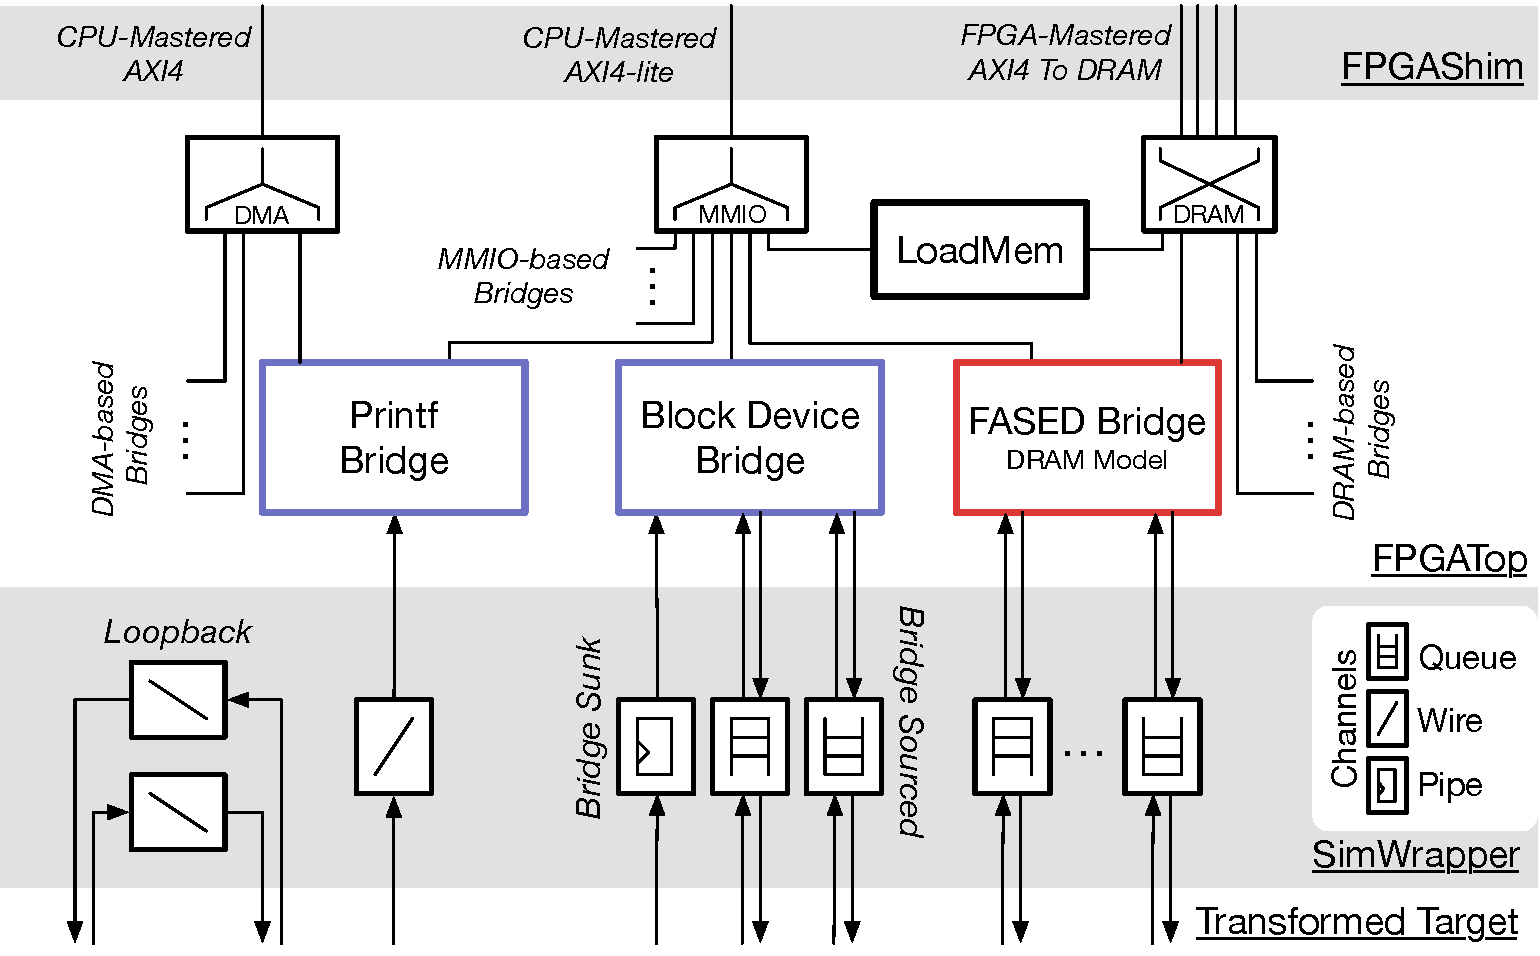
\includegraphics[width=\columnwidth]{figures/sim-wrapper-layers.pdf}
    % graffle2pdf -c wrappers midas-graphics/graffle/sim-wrapper-layers.graffle figures/sim-wrapper-layers.pdf
    \caption{The wrapper circuit generated during platform mapping, with a handful of bridges are shown for
    illustration. The host interfaces at the top (in \texttt{FPGAShim}) match those used in MIDAS. Interconnect
    between host interfaces and bridges initially was identical to that in MIDAS, but has since be augmented.
    Loopback channels, not present in MIDAS, connect two units in the transformed target.
    }
  \label{fig:sim-wrapper-layers}
\end{figure}


\subsection{Channel Synthesis}
The first wrapper layer~(\texttt{SimWrapper}) directly interfaces with the transformed RTL and instantiates
channel implementations. Elaboration of this module is driven by two inputs. First, the user-defined parameters instance
which, as in MIDAS, specifies properties about the host-platform. Second, by
annotations, specifically connection annotations, labelling the now transformed target.
Each connection annotation will corespond with a channel implentation, however how that channel
is bound depends on the \texttt{sources} and \texttt{sinks} enumerated by the annotation.
Connection annotations that posses both \texttt{sources} and \texttt{sinks}
connect two models in the transformed RTL; these are \emph{loopback} channels
that drive an input and an output interface on the transformed target. Conversly,
annotations that possess an empty \texttt{sources} or \texttt{sinks} parameter
are sunk or driven by a bridge module, respectively. In these cases, the
channel implementation has its dequeue or enqueue side
interface exposed to the next wrapper-layer of the module hierarchy.

In all cases, the type of channel generated is parameterized by the
\texttt{channelInfo} field of the connection annotation. Target-decoupled channels, as in
MIDAS, always instantiate a model of a fully decoupled, two-deep queue. Pipe
channels have a configurable latency. Default bridge implementations always
emit channel annotations with latency equal to one to improve FMR, and to maintain the
performance characterisitics of legacy MIDAS simulators. When no additional
models are extracted (i.e., the simulator consists only of the hub unit and
bridges) the expected FMR is identical to MIDAS.
When additional units are extracted, they are always directly wired to the
hub, since the compiler currently cannot find and extract registers~(that is to
say, \texttt{FAMEDefaults} labels these channels as wire-type). This has
the effect of making all multi-model simulators execute with an FMR of at least two\footnote{It is possible to build
simulators with unity FMR, if an optimized model's outputs can runahead. At time
of writing, we have no such implementations.}.

\subsection{Bridge Instantiation}
The next-level of the module hierarchy~(\texttt{FPGATop}) corresponds to the wrapper
circuit generated in MIDAS's platform mapping. I/O on this wrapper module consist of AXI4 interfaces
to drive host-DRAM memory systems, and to support CPU-driven MMIO and DMA.
Instead of using an endpoint map, Golden Gate iterates through each bridge
annotation and reflexively invokes the constructor for the requested
BridgeModule. I/O between the elaborated
bridge instance and the simulation wrapper are connected by looking up the
corresponding channels via their \texttt{globalName} fields.
Resource-interconnect generation is identical to MIDAS's, and for the same
input design, the emitted header is the same. All MIDAS endpoints were ported
to use the new Bridge system, without changing existing host software.

\subsection{Platform Wrapper}
The last level of wrapper module is an FPGA-specific shim layer. The user
selects their desired shim through parameters instance. This serves as an
opportunity to introduce FPGA-specific hardware and modify interface names to
slot into an FPGA shell project. We note that this top-level module could
instantiate all of the IP required to define a complete FPGA project~(as in
SiFive's FPGA shells repository), but none of our shims do so presently. The
class for this wrapper module can be defined outside of Golden Gate and
provided by a user wishing to support a non-standard FPGA.

\section{ICCAD 2019 Golden Gate Publication}

Armed with the machinery to selectively extract and reimplement FPGA-hostile
components of the target design, in our ICCAD2019 we set about optimizing
multi-ported RAMs~(we previously introduced this example in
Section~\ref{sec:iron-law}).  ASIC multi-ported RAMs are a classic culprit of
poor resource utilization in FPGA prototypes, as they cannot be trivially
implemented in BRAM and are instead decomposed into LUTs and
registers~\cite{FPGAGap2}.  While using double-pumping, BRAM duplication, or
FPGA-optimized microarchitectures~\cite{MultiportXOR} can help, here we used Golden Gate to
replace the SRAM with a multi-cycle unit to further reduce resource
utilization. This optimization lets a target memory with $M$ asynchronous read ports and
$N$ write ports to be implemented by time-multiplexing
a single dual-ported BRAM. In contrast to the static time-multiplexing schemes described
by Pellauer et al.~\cite{APortNetworks} and Dwiel et al.~\cite{fabscalarfpga}, our optimization can decouple arbitrary target
memories and replace them with an optimized model without any constraints on the structure or timing of the
target design.

In order to rigoursly verify optimizations, in our ICCAD publication we also
introduced a bounded-model checking flow, called Latency-Insensitive Model
Equivalence~(LIME), hosted in UCLID5~\cite{UCLID5}, to formally verify that
optimized models are valid LI-BDNs implementations of their reference RTL.  Our
manipulations of the module hierarchy were in direct service of this goal, as
any extracted RTL module could trivially serve as the reference RTL for a
verification flow. In our ICCAD paper, we used LIME to verify only our RAM
optimization, however, there is nothing that precludes applying LIME to
\emph{all} reference-unit pairs in a simulator. This verification flow could be
run in parallel to FPGA compilation, providing a multi-hour window to catch
potential bugs before a simulator is deployed to FPGA.

\begin{figure}
  \centering
    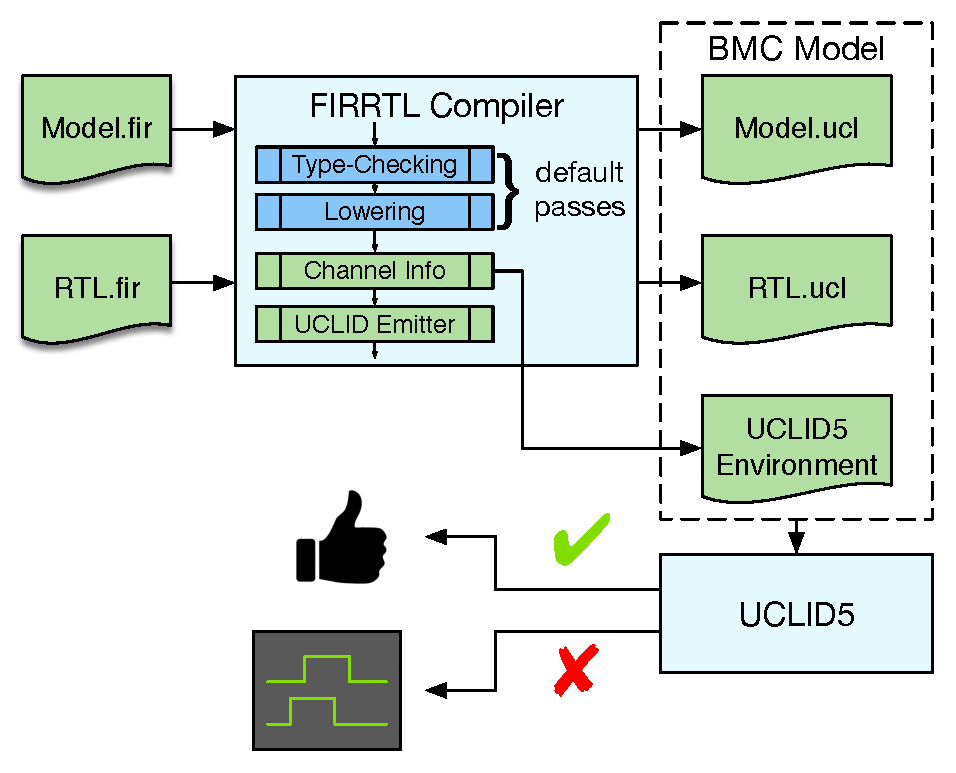
\includegraphics[width=\columnwidth]{figures/lime_flow_small.pdf}
    % -c default midas-graphics/graffle/lime_flow_small.graffle figures/lime_flow_small.pdf
    \caption{The LIME model checking flow. In LIME, FIRRTL for a unit and its
    reference SSM are lowered and emitted as UCLID5 representations. A
    Python-based enironment generator (not shown), consumes channel information
    emitted by the compiler to generate test environments for PI, GC, and NED.
    If the unit is not a valid LI-BDN, LIME produces a waveform counterexample
    that demonstrates how the property under test was violated.
    }
  \label{fig:lime-flow}
\end{figure}


The LIME model checking flow and RAM optimization first described in our
ICCAD2019 paper are primarly contributions of Albert Magyar and are described
at length in Chapters 6 and 7 of his dissertation.

